\question 假定一个磁盘存储器有4个盘片,用于记录信息的柱面数为2000,每个磁道上有3000个扇区,每个扇区512B,则该磁盘存储器的容量约为(
)。(取1G=10\^{}9)
\par\twoch{12MB}{24MB}{12GB}{\textcolor{red}{24GB}}
\begin{solution}一片硬盘盘片有正反两面,4个盘片,也就是有8个盘面。那么该磁盘存储器的容量计算如下:
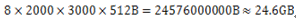
\includegraphics[width=3.08333in,height=0.22917in]{computerassets/475e8ad55ad674b91daa77dfdef019ad.png}
选项中,最接近的答案为D。
\end{solution}
\question 为提高存储器的存取效率,在安排磁盘上信息分布时,通常是
\par\twoch{存满一面,再存另一面}{尽量将同一文件存放在一个扇区或相邻扇区的各磁道上}{\textcolor{red}{尽量将同一文件存放在不同面的同一磁道上}}{上述方法均有效}
\begin{solution}磁盘各记录面上相同编号(位置)的磁道称为一个圆柱面。当主机存放文件时,应尽可能地将它存放在同一圆柱面中。这是因为在同一圆柱面上由于各记录面的磁头已同时定位,换道的时间只是磁头选择电路的译码时间,速度很快。如果选择同一记录面上的不同磁道,则每次换道时都要进行磁头定位操作,速度较慢。
\end{solution}
\question 设一个磁盘盘面共有200个磁道,盘面总存储容量60MB,磁盘旋转一周的时间为25ms,每磁道有8个扇区,各扇区之间有一间隙,磁头通过每个间隙需1.25ms。则磁盘通道所需最大传输率是
\par\twoch{10MB/s}{60MB/s}{83.3MB/s}{\textcolor{red}{20MB/s}}
\begin{solution}每个磁道的容量=60MB/200=0.3MB,读一个磁道数据的时间等于磁盘旋转一周的时间减去经过扇区之间的间隙的时间(每磁道有8个间隙),即读一个磁道数据的时间=25ms-
1.25ms×8=15ms,磁盘的数据传输率=0.3MB/15ms=0.3MB/0.015s=20MB/s。
\end{solution}
\question 对于磁盘来说,扇区的编号方式直接影响磁盘数据的读写时间。若磁头转过一个扇区的时间为t,磁盘读取一个扇区的时间为1.5t,那么下列磁盘编号方式中,具有最好性能的编号方式是
\par\fourch{}{}{\textcolor{red}{}}{}
\begin{solution}磁盘每当访问一个逻辑扇区后,需等待主机将该扇区的输出数据处理完毕后才能进行下一个扇区的读写。在这个等待过程中,硬盘可能已经转过了几个物理扇区。因此我们需要进行交叉编号,而本题磁盘读取一个扇区后,磁头是转过1.5个扇区了。也就是下一个编号应该是此时磁头最接近的下一个扇区。
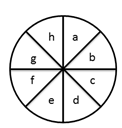
\includegraphics[width=1.27083in,height=1.33333in]{computerassets/67e305368a3f1c270fc41c3ae1aa9924.png}
例如上图中,若磁盘读取了a扇区后,磁头应该是处于c扇区中间位置的,那么理想情况下,下一个读取的扇区就应该是d扇区(因为c扇区已经过了一半了),因此扇区a和d的编号应该是连续的。依次类推,每两个连续逻辑扇区之间所间隔的物理扇区数为2,本题的C选项最满足题意,因此本题选C。
\end{solution}
